\addcontentsline{toc}{section}{Compatibility matrix of displacements}
\section*{Compatibility matrix of displacements}
It's based on the discrete model. It represents a relationship among the local
and global displacements. We used 4 finite elements for each one has 6 local
displacement and 5 nodes have total number of global displacements m=16. The
final compatibility matrix of displacements are shown on figure
\ref{fig:CDmatrix}, where rows are global displacements and columns are local
displacements.
\begin{figure}[H]
  \centering
  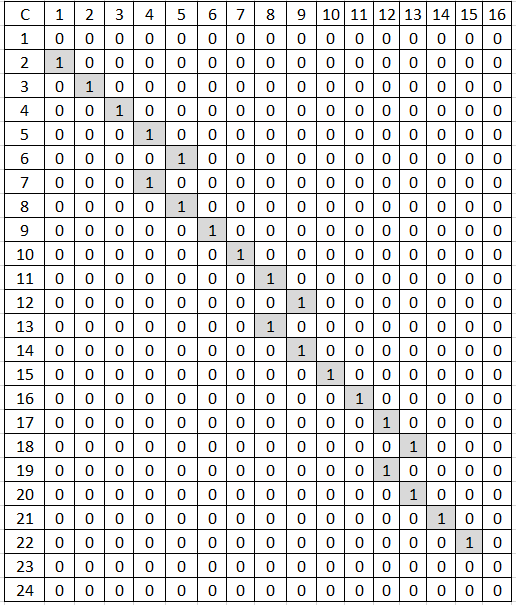
\includegraphics[width=0.5\textwidth]{./fig/CDmatrix.png}
    \caption{Mitral valve structure}
    \label{fig:CDmatrix}
\end{figure}
%\VerbatimInput[fontsize=\fontsize{7}{9}\selectfont]{Cmtxoutput.txt}